\chapter{Risultati}
\label{ch:risultati}

In questo capitolo vengono presentati i risultati ottenuti durante la fase di
benchmarking della libreria e della procedura \texttt{gain}, ovvero quella
soggetta alle ottimizzazioni nel capitolo precedente. Questa fase è di notevole importanza,
in quanto permette di valutare il lavoro svolto, confrontando tutti i framework di
parallelizzazione tra loro, oltre che all'implementazione originale, per avere un
quadro completo del prodotto finale.

\section{Metodologia di valutazione}
\label{sec:bencharmking}

Per poter valutare le prestazioni della libreria sono stati eseguiti diversi
test di benchmarking che hanno permesso di confrontare tra loro le prestazioni, i
miglioramenti e le differenze delle diverse soluzioni. Inoltre, è stato fondamentale
valutare la correttezza matematica della procedura modificata per assicurarsi che
non siano stati introdotti errori durante la fase di sviluppo, per tutti e tre i
framework di parallelizzazione. In merito allo svolgimento, la libreria \textit{CoopeRIS}
è dotata di un insieme di \textit{unit test} che sono stati eseguiti per
garantirlo. Tutte le misurazioni delle tempistiche sono state eseguite su macchine
con diverse configurazioni hardware per poter valutare le prestazioni in scenari
differenti.

\section{Benchmarking della libreria}
\label{sec:benchmarking}

Il benchmarking della procedura ottimizzata e della libreria è stato eseguito
senza la necessità di alcuno dei framework esterni citati nel capitolo
\ref{subsec:risframework}. Questo è stato essenziale per poter valutare le prestazioni
in modo puro e indipendente. Per fare ciò, è stato creato un programma molto semplice,
che ha eseguito ripetutamente le procedure sotto esame, misurando tramite la libreria
\textit{chrono} di C++ il tempo di esecuzione di ciascuna di esse. Il programma è
stato eseguito su diverse macchine, soprattutto per poter valutare situazioni
con un elevato numero di core CPU. Per garantire una maggiore precisione,
ciascuna misurazione è stata eseguita più volte, da un minimo di dieci fino ad un
massimo di mille, per calcolarne la media ed eliminare eventuali errori dovuti a
fluttuazioni dell'ambiente di esecuzione.

\subsection{Risultati complessivi}
\label{subsec:risultati-complessivi}

I risultati complessivi del benchmarking della libreria sulla procedura \texttt{gain}
sono stati molto positivi. Le ottimizzazioni apportate hanno ottenuto un notevole
incremento prestazionale, raggiungendo in alcuni casi un aumento fino a due
ordini di grandezza nei casi in cui le RISs presentavano il numero massimo di
elementi supportati. Nelle figure \ref{fig:risultati-complessivi} e \ref{fig:risultati-complessivi-log}
sono riportate le misurazioni del tempo di esecuzione, rispettivamente in scala
lineare e scala logaritmica per una miglior visualizzazione dei dati, in funzione
del numero di elementi della RIS simulata. I punti rappresentano rispettivamente
i tempi campionati di esecuzione della procedura non ottimizzata e della
procedura ottimizzata tramite multi-threading, OpenCL e CUDA, mentre le linee
tratteggiate rappresentano il fit dei dati. L'interesse principale di quest'ultime
è quello di valutare l'effettiva linearità in termini di complessità del problema
e per individuare eventuali punti in cui l'aggiunta di procedure lineari per implementare
la parallelizzazione possano aver introdotto un overhead non trascurabile. In
figura \ref{fig:perc-better} è riportata la percentuale di tempo di esecuzione
rispetto all'impostazione originale rispetto al numero di elementi della RIS. Tutti
i test dimostrano una chiara superiorità delle soluzioni che sfruttano il calcolo
parallelo, con le implementazioni su GPU che ottengono un tempo di esecuzione da
l'\textit{1,2\%} all'{1,6\%} rispetto all'implementazione originale, mentre per
quella su CPU si ottengono valori che variano dal \textit{10,2\%} al \textit{13,3\%},
perfettamente in linea con l'ideale \textit{12,5\%} di miglioramento atteso. I benchmark
sono stati eseguiti su una macchina con processore Intel Core i7-8700K, con 8
core fisici e NVIDIA GeForce GTX 1080.

\begin{figure}[!ht]
  \centering
  \subfloat[
  \centering
  scala lineare]{{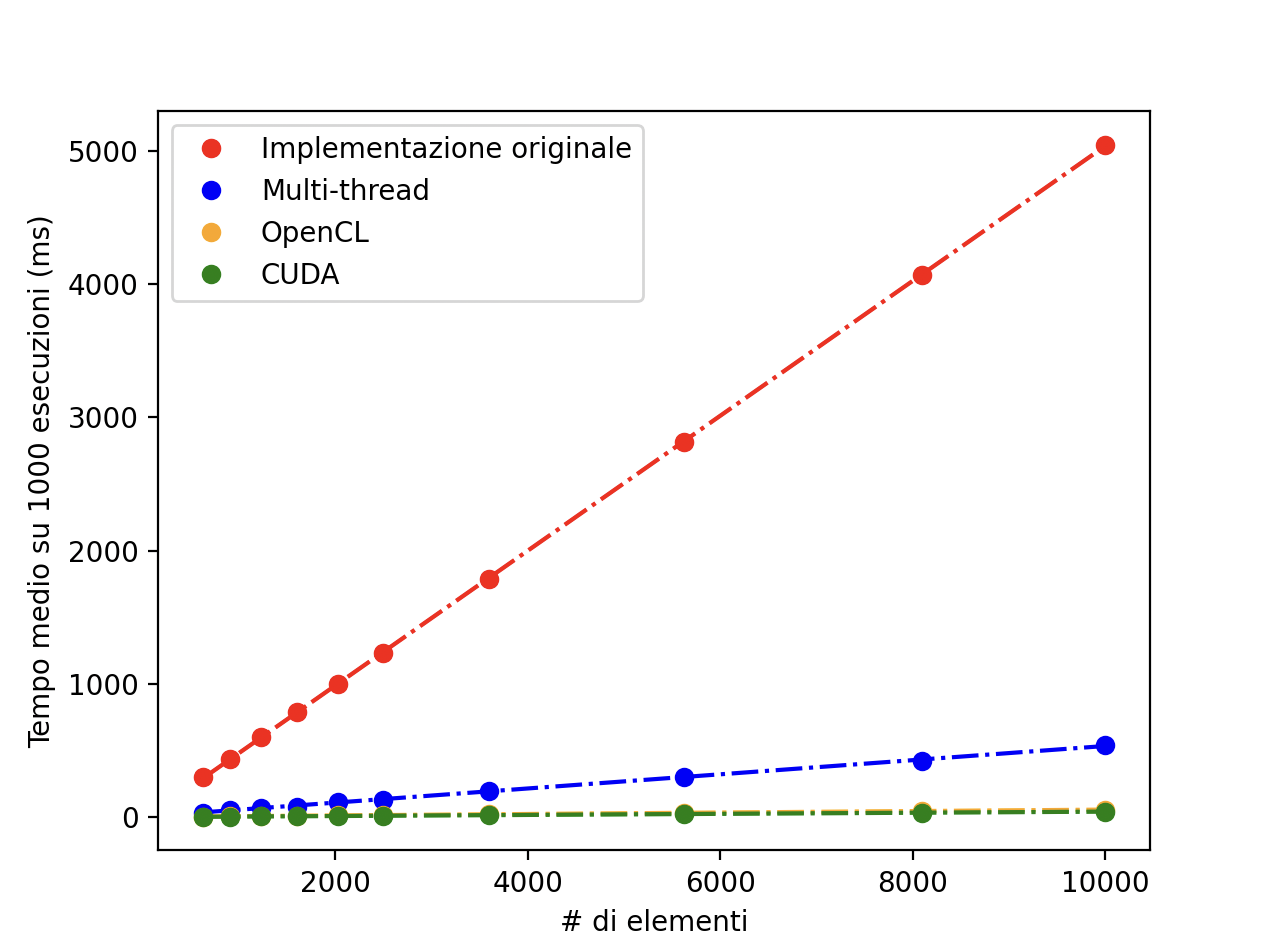
\includegraphics[width=8cm]{images/results/gain-over-elem.png}\label{fig:risultati-complessivi}}}
  \subfloat[
  \centering
  scala logaritmica]{{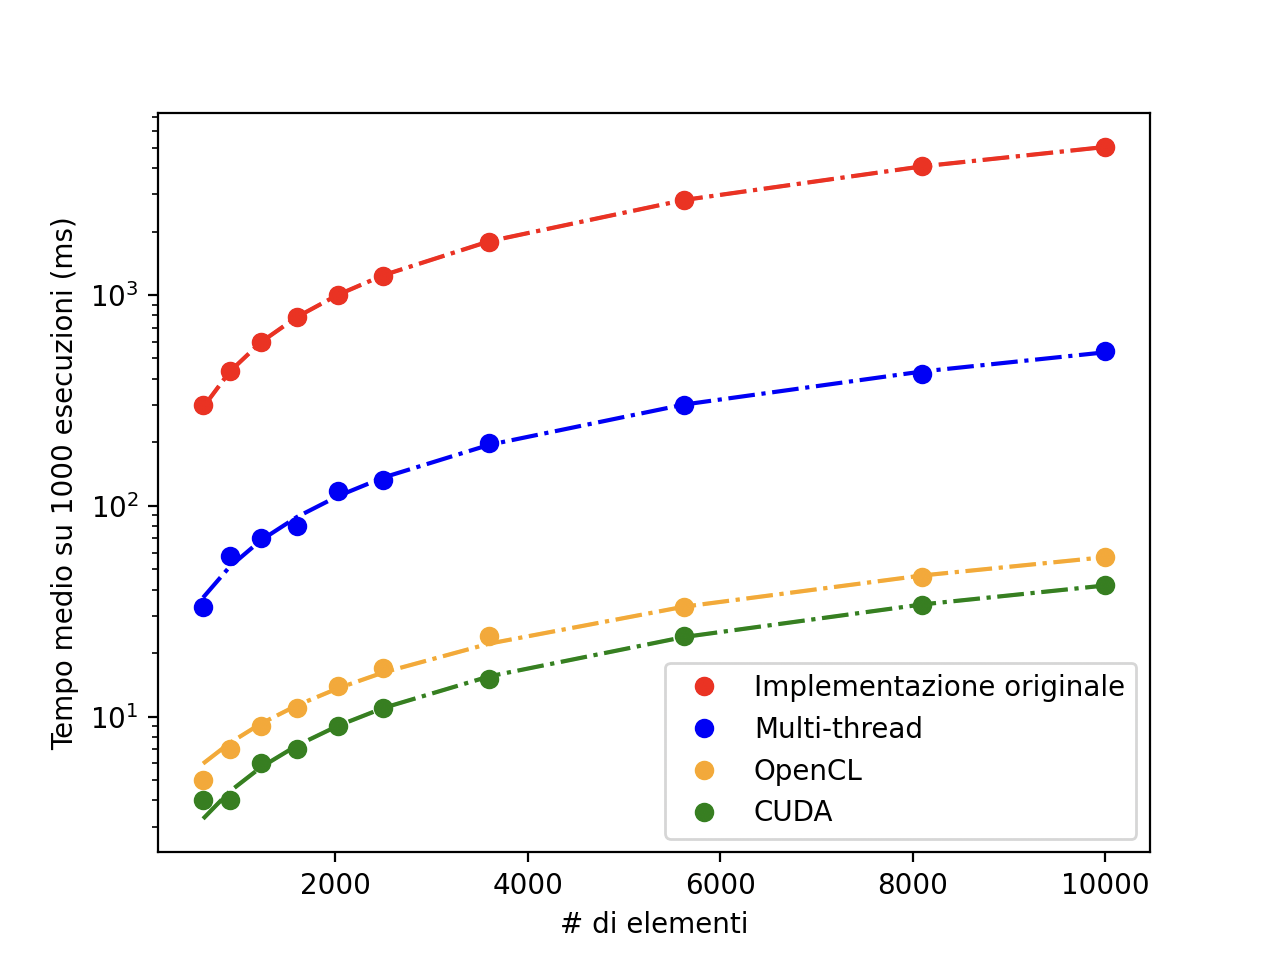
\includegraphics[width=8cm]{images/results/gain-log-over-elem.png}\label{fig:risultati-complessivi-log}}}
  \caption{Risultati complessivi del benchmarking}
\end{figure}

\begin{figure}[!ht]
  \begin{minipage}[t]{0.5\linewidth}
    \centering
    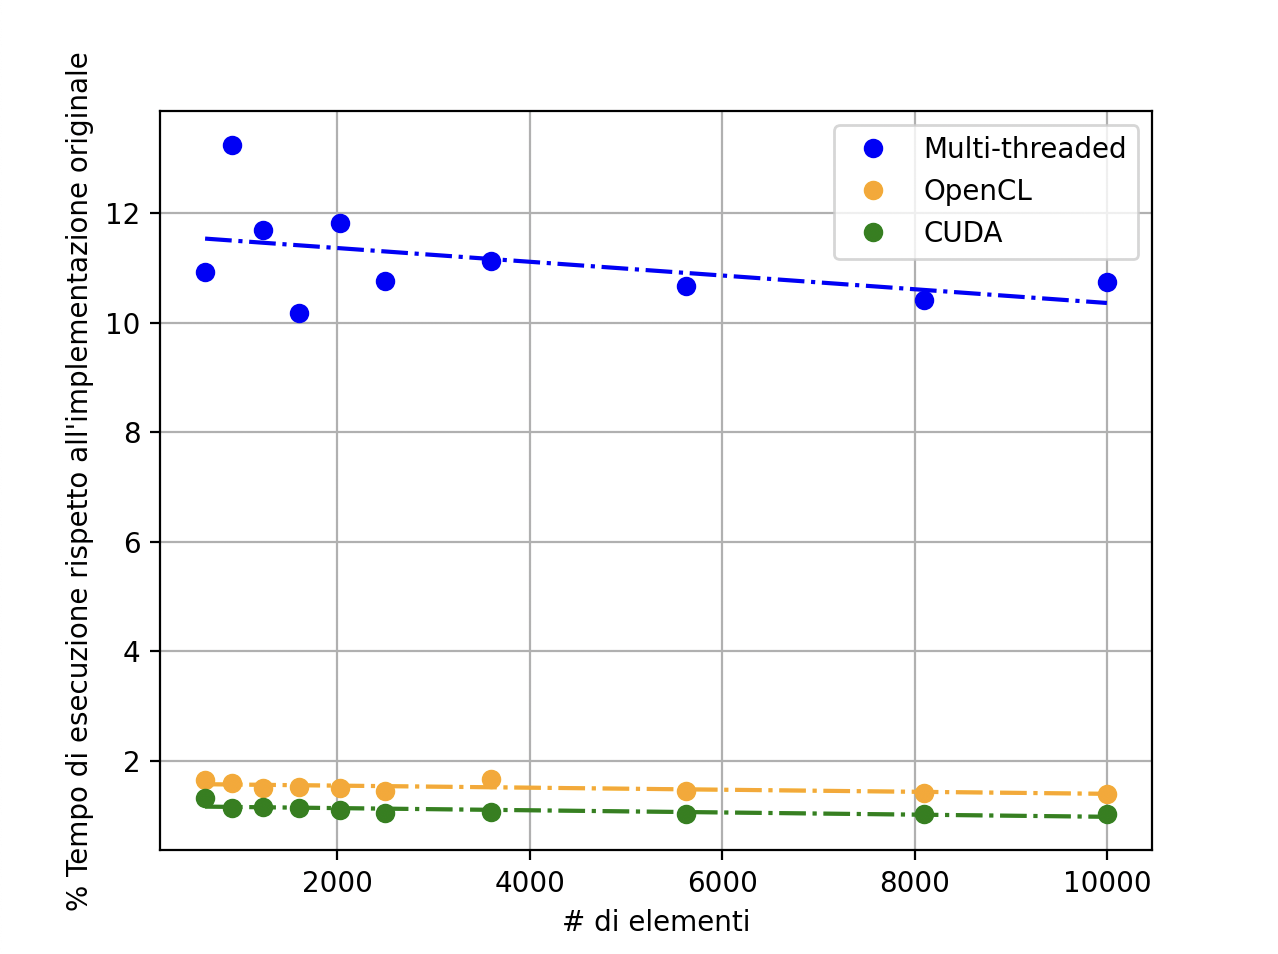
\includegraphics[width=8cm]{images/results/gain-perc-better.png}
    \begin{adjustwidth}
      {0pt}{5pt}
      \begin{varwidth}
        {8cm}
        \caption{Percentuale di tempo di esecuzione rispetto all'impostazione
        originale}
        \label{fig:perc-better}
      \end{varwidth}
    \end{adjustwidth}
  \end{minipage}
  \begin{minipage}[t]{0.5\linewidth}
    \centering
    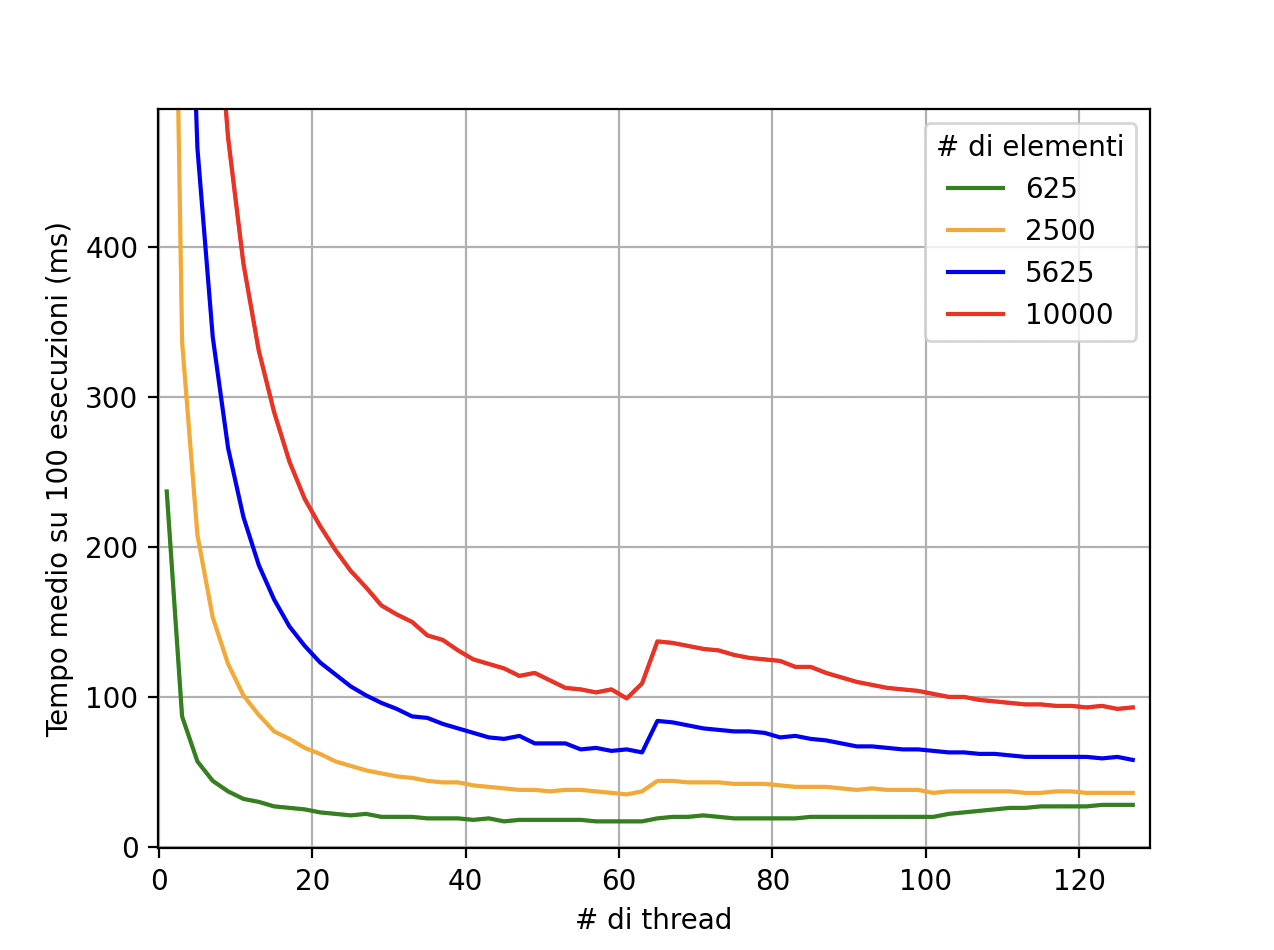
\includegraphics[width=8cm]{images/results/gain-comp-threads.png}
    \begin{adjustwidth}
      {0pt}{5pt}
      \begin{varwidth}
        {8cm}
        \caption{Comparazione performance tra diverso numero di thread}
        \label{fig:risultati-cpu}
      \end{varwidth}
    \end{adjustwidth}
  \end{minipage}
\end{figure}

\subsection{Risultati: CPU single-thread vs multi-thread}
\label{subsec:risultati-cpu}

Particolare attenzione è stata posta nel confronto tra l'implementazione
originale e multi-thread. Molteplici test e benchmark sono stati eseguiti per valutare
le prestazioni con diversi numeri di thread CPU. In figura
\ref{fig:risultati-cpu} sono riportati i risultati ottenuti al variare del
numero di thread utilizzati per quattro delle configurazioni di elementi RISs, nello
specifico \textit{625}, \textit{2500}, \textit{5625} e \textit{10000} elementi.
Si evince chiaramente come la soluzione multi-thread, ad un numero di thread molto
elevato, saturi le prestazioni della CPU e non permetta di ottenere ulteriori
incrementi prestazionali, dovuto al crescente overhead introdotto per processare
i risultati parziali dei thread, oltre al costo di creazione e gestione dei
thread stessi. Il caso più interessante è quello con \textit{625} elementi, dove
si può osservare chiaramente come da circa \textit{60} thread in poi, il costo di
un ulteriore thread peggiori le prestazioni della procedura, rendendo quindi
inutile ogni ulteriore incremento. Si noti inoltre come, superata la soglia dei
\textit{65} thread, si verifichi un fenomeno dove l'aggiunta di un thread che
necessariamente deve essere eseguito tramite \textit{hyperthreading}, riduca la
performance generale della procedura. Invece, in figura
\ref{fig:jobs-per-thread} è riportato il confronto tra la grandezza dei dati da
elaborare per thread, al variare del numero di thread utilizzati. Si ritrova
anche qui lo stesso fenomeno di diminuzione delle prestazioni dovuto all'\textit{hyperthreading}.
Per concludere, in figura \ref{fig:thread-over-elem} è riportato il confronto tra
il numero di elementi RISs e il numero di thread utilizzati, in scala
logaritmica. Anche qui, la linea tratteggiata rappresenta il fit dei dati, che evidenzia
l'effettiva linearità del problema e la corretta scalabilità della procedura.
Inoltre, si osserva come, nei casi con numero di elementi RISs basso, le misurazioni
con numero massimo di thread siano leggermente inferiori rispetto a quelle con un
numero minore, evidenziando l'overhead introdotto da questo tipo di
parallelizzazione. Questi dati sono di fondamentale importanza per poter valutare
il numero ottimale di thread da utilizzare per ottenere le migliori prestazioni possibili.
I test in riferimento sono stati eseguiti su una macchina con processore AMD
Ryzen Threadripper 3990X, con 64 core fisici e 128 thread per le figure \ref{fig:risultati-cpu}
e \ref{fig:jobs-per-thread}, mentre per la figura \ref{fig:thread-over-elem} su
2x Intel Xeon E5-2680 v4, con 14 core fisici e 28 thread, quindi 56 thread in
totale.

\begin{figure}[!ht]
  \begin{minipage}[t]{0.5\linewidth}
    \centering
    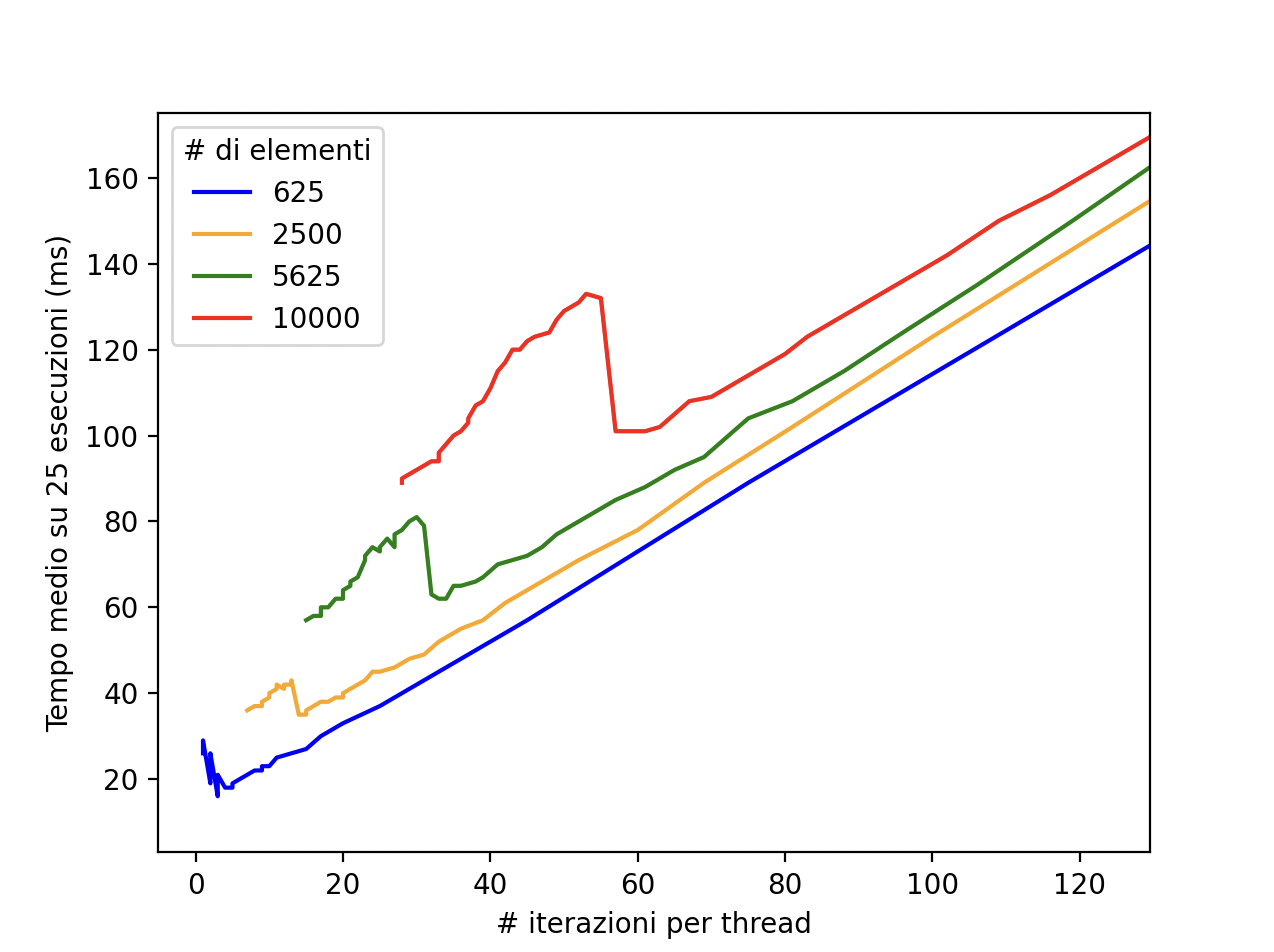
\includegraphics[width=8cm]{images/results/gain-jobs-per-thread.png}
    \begin{adjustwidth}
      {5pt}{0pt}
      \begin{varwidth}
        {8cm}
        \caption{Comparazione per grandezza di dati da computare per thread}
        \label{fig:jobs-per-thread}
      \end{varwidth}
    \end{adjustwidth}
  \end{minipage}
  \begin{minipage}[t]{0.5\linewidth}
    \centering
    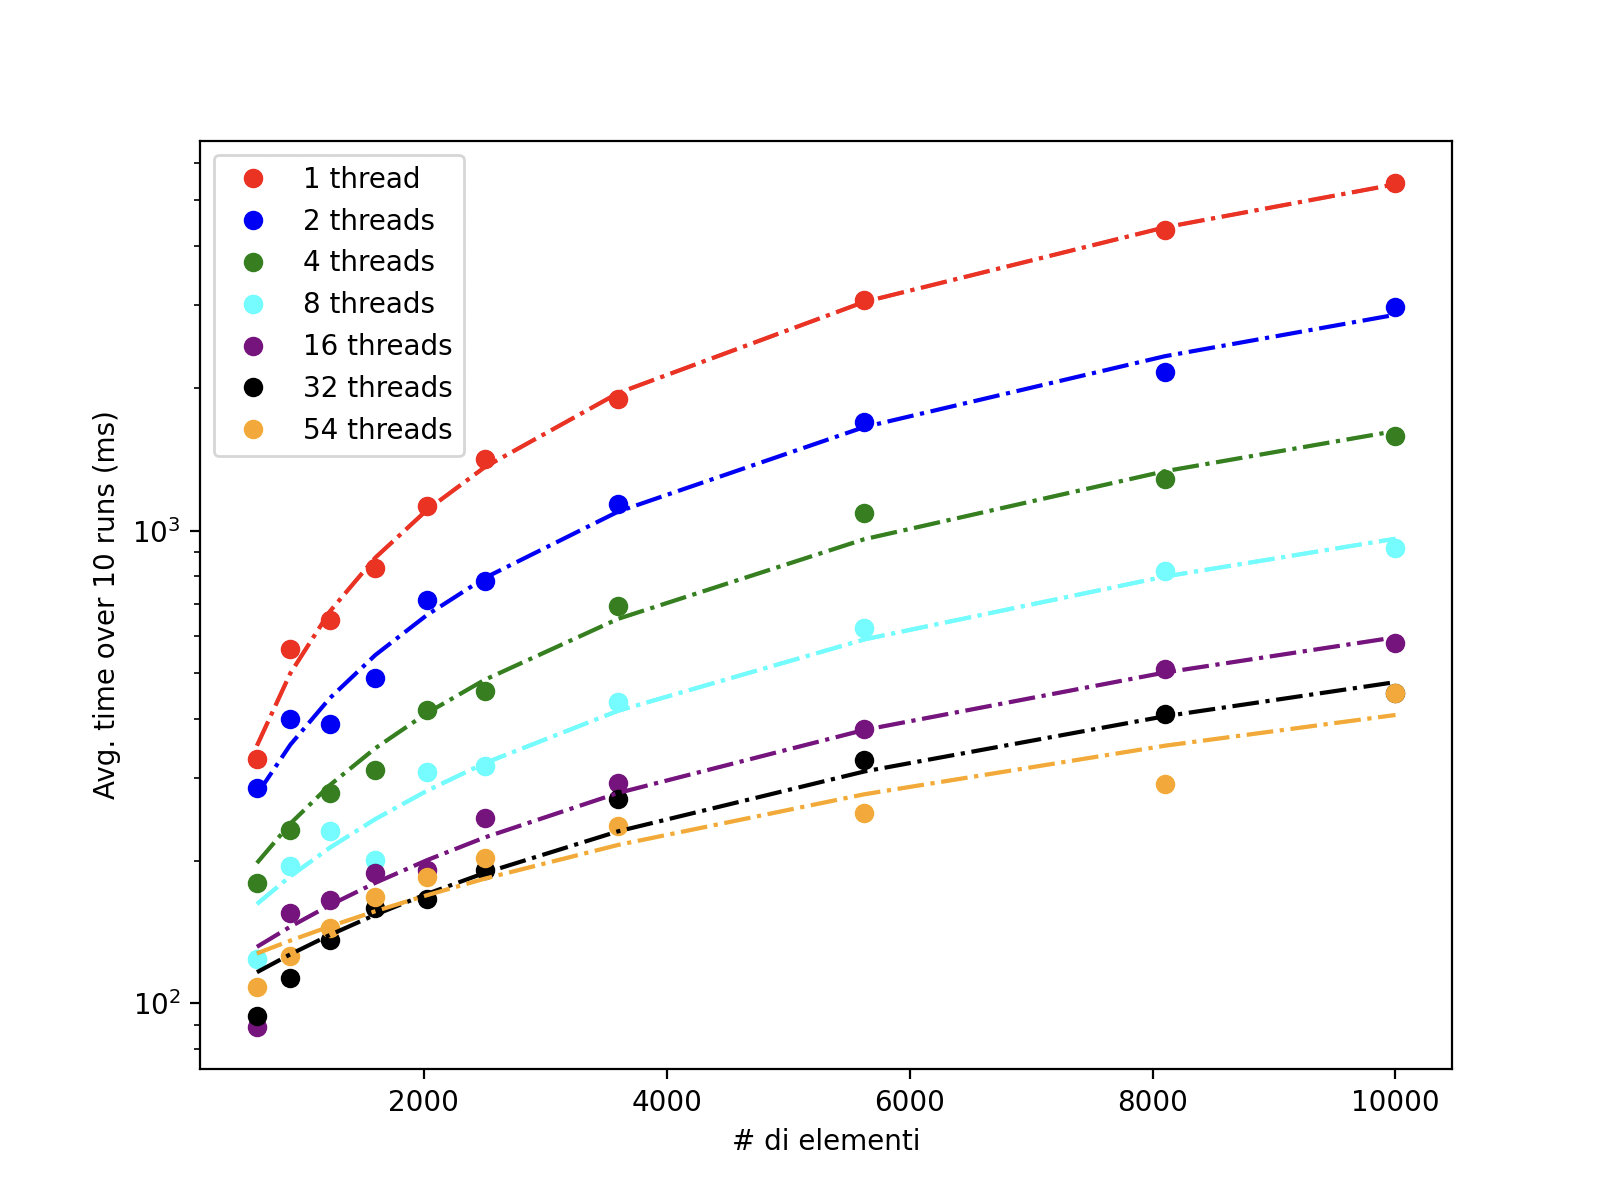
\includegraphics[width=8cm]{images/results/gain-thread-over-elem.png}
    \begin{adjustwidth}
      {5pt}{0pt}
      \begin{varwidth}
        {8cm}
        \caption{Comparazione per thread al variare del numero di elementi RISs}
        \label{fig:thread-over-elem}
      \end{varwidth}
    \end{adjustwidth}
  \end{minipage}
\end{figure}

\subsection{Risultati: CUDA vs OpenCL}
\label{subsec:risultati-cuda-opencl}

In figura \ref{fig:risultati-cuda-opencl} si trova la comparazione percentuale
delle prestazioni dei framework GPU al variare del numero di elementi RISs. La baseline
al \textit{100\%} rappresenta il tempo di esecuzione della procedura tramite
CUDA allo specifico numero di elementi. Si può osservare come l'implementazione tramite
CUDA sia leggermente più performante rispetto a quella tramite OpenCL, con una
diminuzione prestazionale che varia dal 20\% al 37,5\%. Inoltre, nella
misurazione è stato volutamente omesso il tempo di inizializzazione degli
oggetti \textit{ReconfigurableIntelligentSurface}, che in OpenCL comprende la
compilazione del kernel della funzione \texttt{gain} a runtime, poiché è un'operazione
che viene eseguita una sola volta all'avvio del framework e non impattante nel
contesto generale di una simulazione. I risultati sono stati ottenuti su una macchina
con scheda grafica NVIDIA GeForce GTX 1080.

\begin{figure}[!ht]
  \begin{minipage}[t]{0.5\linewidth}
    \centering
    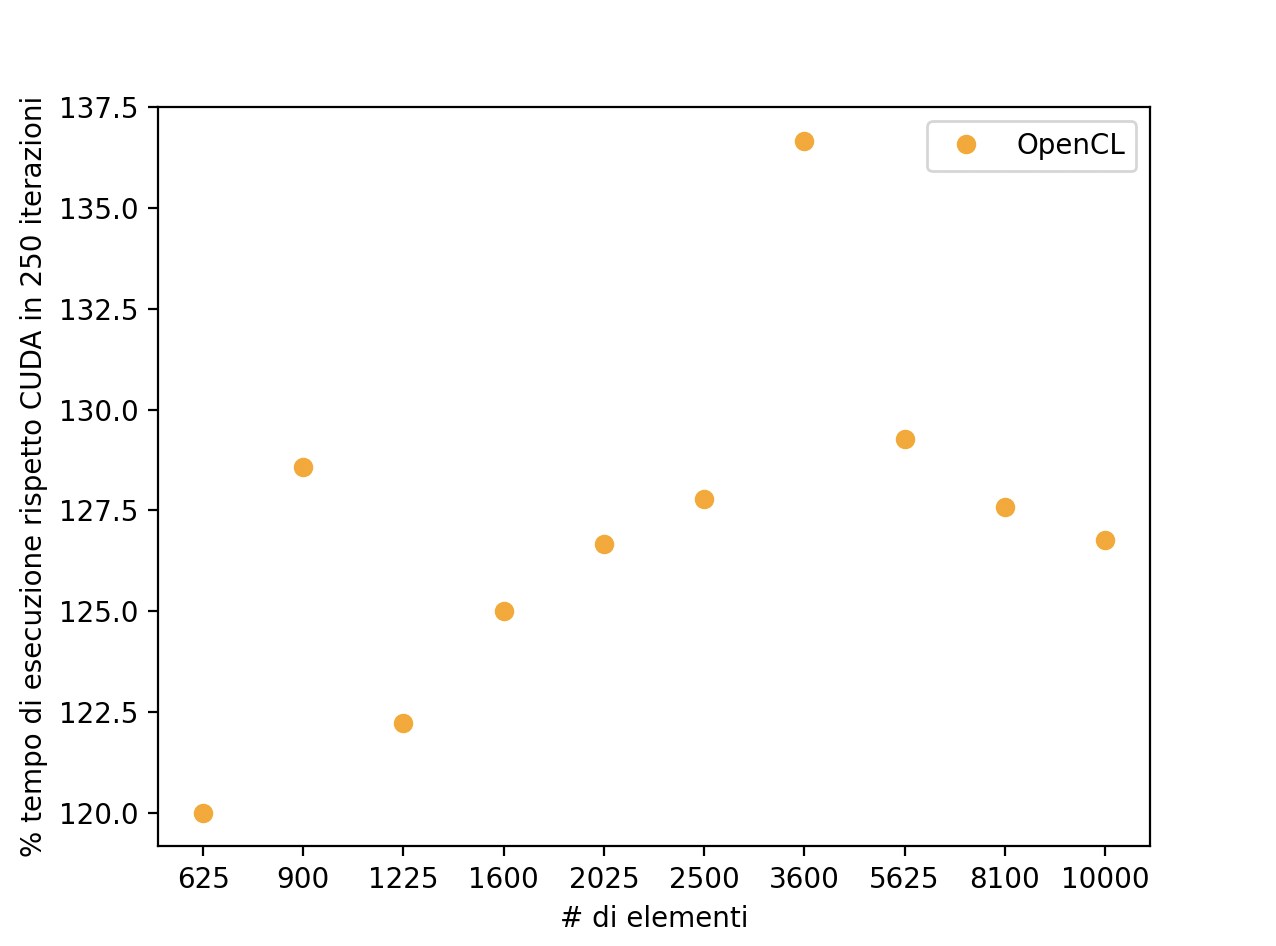
\includegraphics[width=8cm]{images/results/gain-cuda-vs-opencl.png}
    \begin{adjustwidth}
      {0pt}{5pt}
      \begin{varwidth}
        {8cm}
        \caption{Differenza percentuale tra CUDA e OpenCL}
        \label{fig:risultati-cuda-opencl}
      \end{varwidth}
    \end{adjustwidth}
  \end{minipage}
  \begin{minipage}[t]{0.5\linewidth}
    \centering
    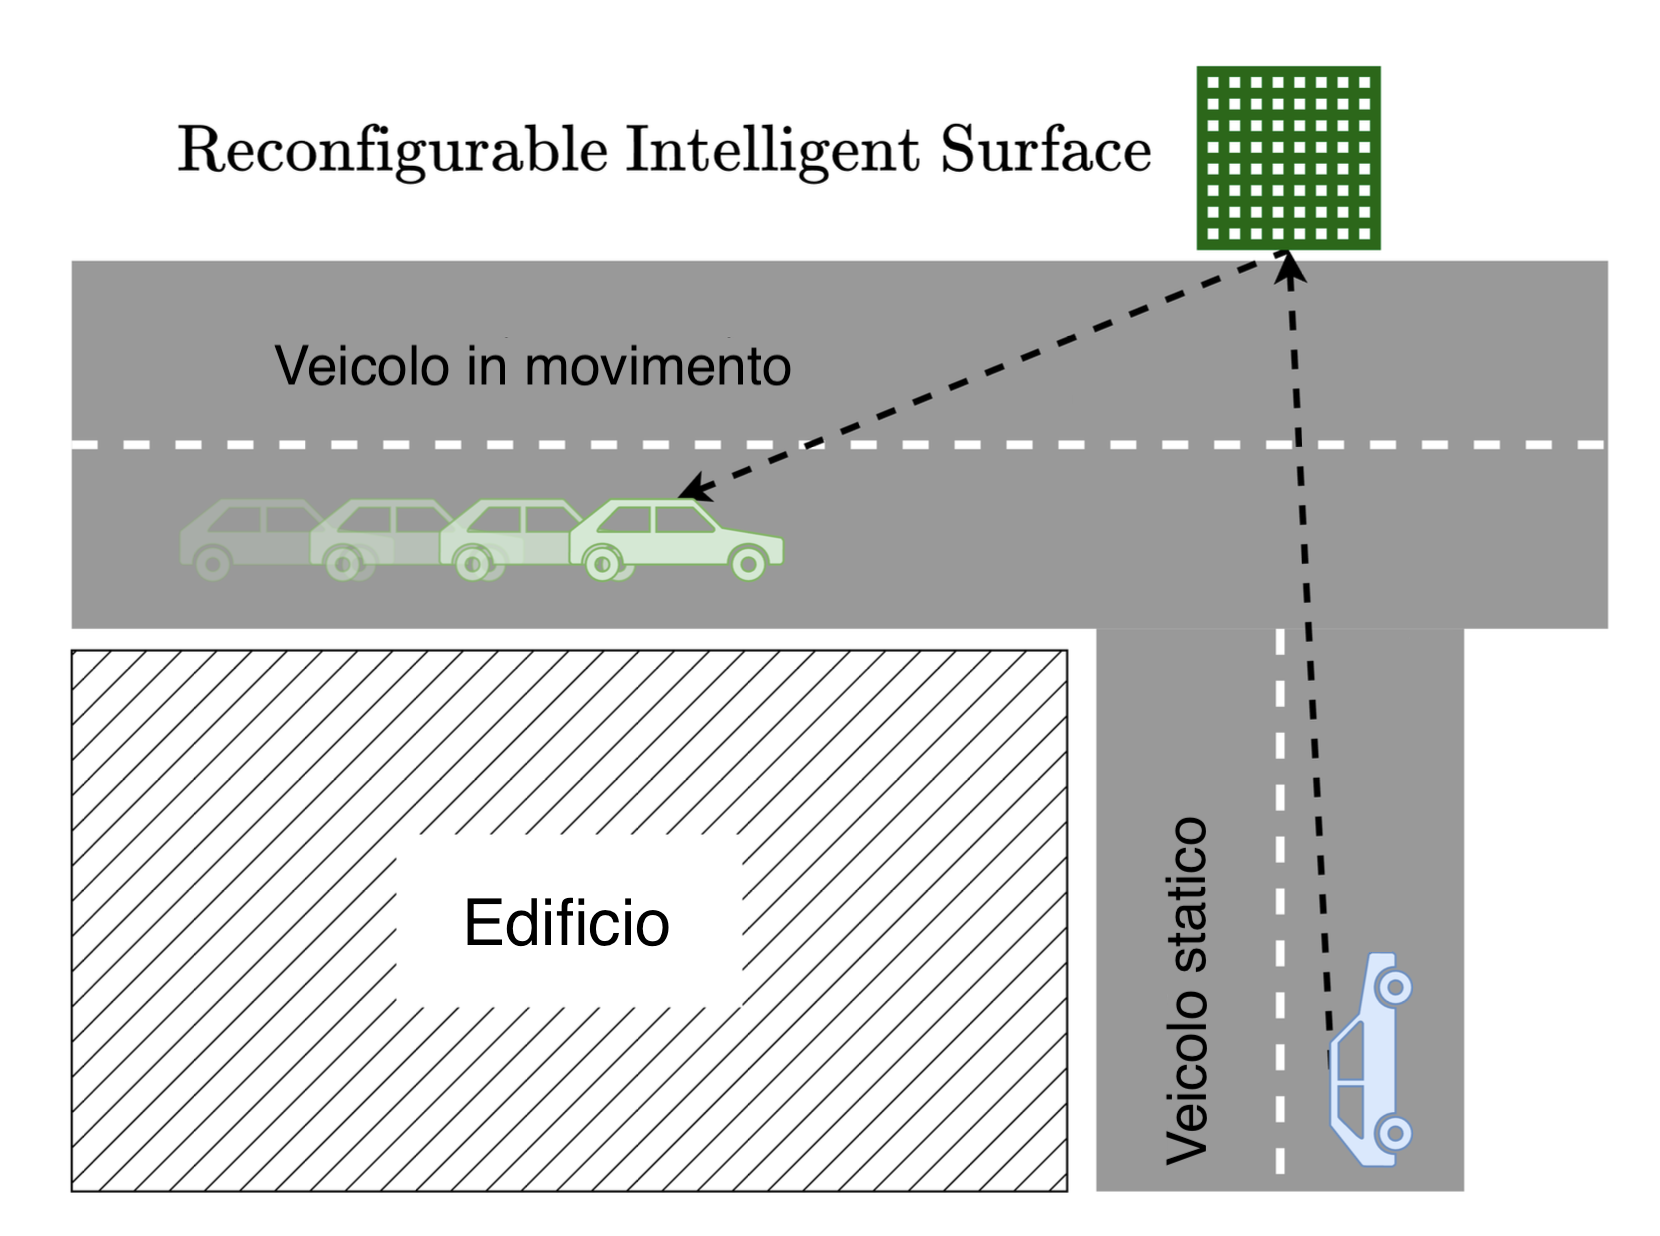
\includegraphics[width=8cm]{images/examples/framework-example.png}
    \begin{adjustwidth}
      {5pt}{0pt}
      \begin{varwidth}
        {8cm}
        \caption{Scenario di esempio del framework\cite{cooperis}}
        \label{fig:framework-scenario}
      \end{varwidth}
    \end{adjustwidth}
  \end{minipage}
\end{figure}

\vfill

\section{Dimostrazione di una simulazione sul framework}
\label{sec:dimostrazione}

Come dimostrazione finale, si vogliono portare i risultati delle simulazioni
tramite tutte le implementazioni della libreria, compresa quella originale, all'interno
del framework nello scenario di esempio raffigurato in figura
\ref{fig:framework-scenario}. Esso consiste in una RIS e un edificio che separa due
veicoli, uno in movimento e l'altro fermo, che comunicano tramite un canale che non
sarebbe possibile senza l'ausilio della RIS data la presenza dell'edificio. Gli
esiti delle misurazioni, consultabili nelle figure \ref{fig:risultati-framework}
e \ref{fig:risultati-framework-log} rispettivamente in scala lineare e logaritmica,
sono completamente in linea con quelli ottenuti durante il benchmarking della
libreria. Specificamente, si rilevano incrementi prestazionali da un minimo di
37 volte fino ad un massimo di 80 nel caso in cui la RIS possedeva il numero
massimo di elementi supportati tramite parallelizzazione su GPU, e un miglioramento
di circa 8 volte per tutte le configurazioni della RIS tramite parallelizzazione
su CPU, perfettamente lineare con il numero di thread utilizzati considerando il
tempo di inizializzazione dei framework. Questi risultati denotano pienamente l'efficacia
dell'implementazione di soluzioni tramite calcolo parallelo apportate alla libreria,
e la loro applicabilità in scenari reali. Le simulazioni sono state eseguite su una
macchina con processore Intel Core i7-8700K, con 8 core fisici e NVIDIA GeForce
GTX 1080.

\begin{figure}[!ht]
  \centering
  \subfloat[
  \centering
  scala lineare]{{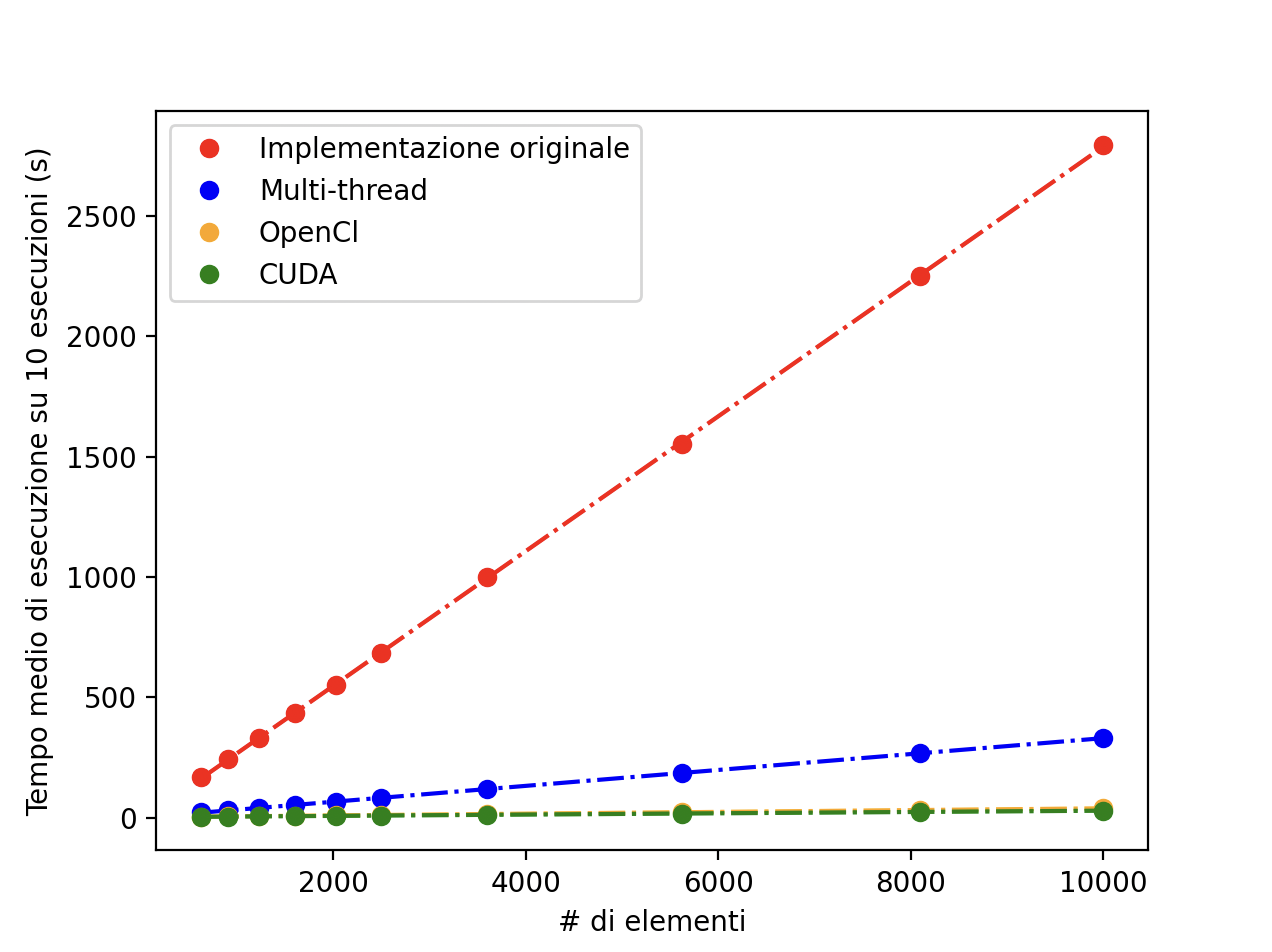
\includegraphics[width=8cm]{images/results/framework-over-elem.png}\label{fig:risultati-framework}}}
  \subfloat[
  \centering
  scala logaritmica]{{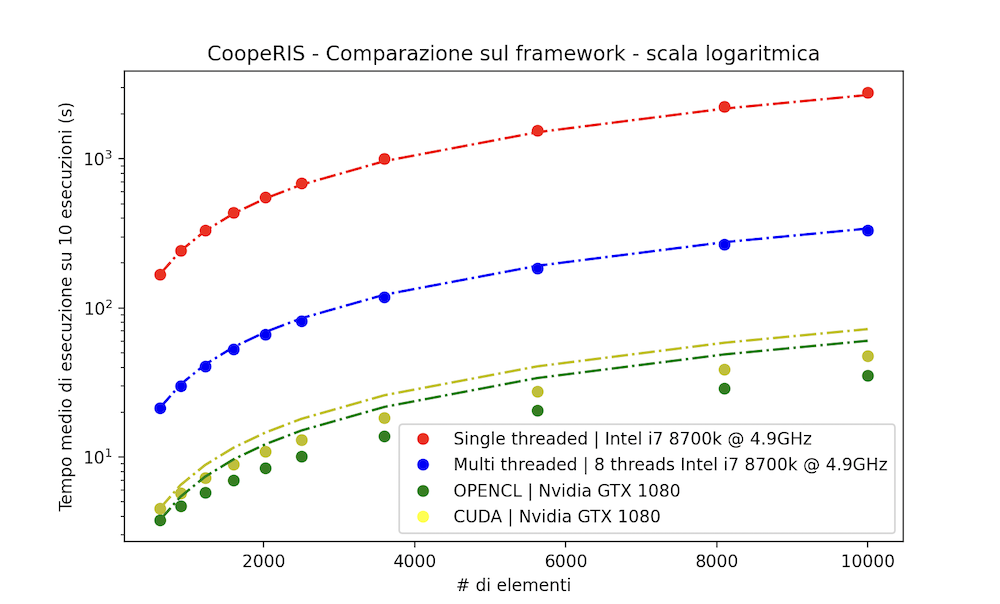
\includegraphics[width=8cm]{images/results/log-framework-over-elem.png}\label{fig:risultati-framework-log}}}
  \caption{Risultati del benchmarking su una simulazione reale tramite il
  framework}
\end{figure}